\documentclass{article}
\usepackage{graphicx}
\begin{document}
\section*{Introduction}
\subsection*{Digital Audio}
Sound, in nature is a continuous variation in pressure over time. 
These pressure 'waves' are incident on the ear and this ends up being perceived 
as sound. This is called Analogue audio. Before going into working with digital 
audio, i would like to touch upon the process in which these sound waves are 
stored in the computer. The most basic of all signals, the sine wave. This can 
represent a sound.
\begin{figure}[h]
\begin{center}
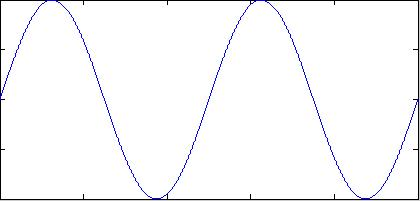
\includegraphics[height=80pt]{../pictures/image1.jpg}
\end{center}
\end{figure}
\newline \\ Now this is an analouge sound i.e., this is nature, not numbers. But a computer 
can work only with numbers. So, we measure the amplitude of the above wave at 
regular intervals. These intervals are evenly spaced over time. This process is called sampling. 
\newline \\ The result looks somewhat like this.
\begin{figure}[h]
\begin{center}
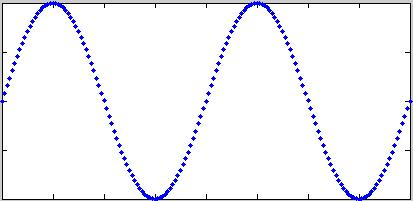
\includegraphics[height=80pt]{../pictures/image2.jpg}
\end{center}
\end{figure}
\newline \\ Each of those dots are the points of the original wave that we measured. Obviously, 
we know the amplitude at each of those points (essentially, a number) and hence 
we can store this in the computer. This kind of dot-like signal is called a 
discrete signal. We can always reconstruct the original signal by simply 
'joining the dots' of this discrete signal.
\subsubsection*{Sampling frequency}
Remember now that we simply have a stream of amplitude values. 
Also remember that I emphasized on the phrase 'evenly spaced in time'.
What this means is, the number of measurements you make in a second is a constant quantity. 
The more number of measurements you make in a second, the closer together are the dots. 
Intuitively, this would be a better approximation to the analogue signal. This 
'the number of measurements you make in a second' is called the sampling frequency. 	
\begin{figure}[h]
\begin{center}
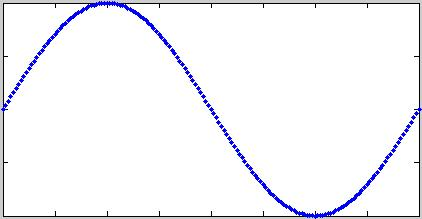
\includegraphics[height=80pt]{../pictures/image101.jpg}
\end{center}
\end{figure}
\newline \\ It is usually around 44100Hz for audio. Either way, this is an important parameter 
when converting any analogue signal to digital.
\section*{A Basic Delay Block}
\begin{figure}[h]
\begin{center}
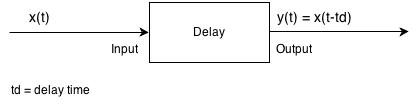
\includegraphics[height=80pt]{../pictures/image3.jpg}
\end{center}
\end{figure}
That block is basically delaying the signal by ts. 
\newline \\ \texttt{x(t)} is an array containing the input signal
\newline \\ \texttt{y(t)} is the output signal (which is nothing but the delayed input signal)
\newline \\This can be implimented in a simple for loop, looping over all the contents of x. 
\section*{A Fed-Back Delay Block}
If you want your delay to repeat at regular intervals, you make an additional feedback loop.
\begin{figure}[h]
\begin{center}
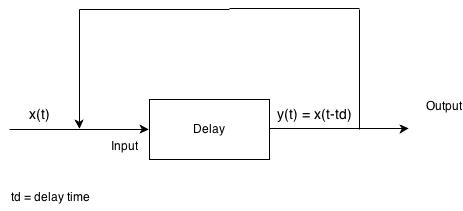
\includegraphics[height=120pt]{../pictures/image4.jpg}
\end{center}
\end{figure}
\newline \\That way, your delayed output is once again fed back to the input, 
this causes it to get delayed again by the same amount of time, ad infinium 
(or as long as your for loop lets you). Notice that the input to the delay 
block is actually something like:
\newline \\ \texttt{x(t) + y(t)}
\newline \\ And the output must be a delayed version of this:
\newline \\ \texttt{x(t-ts) + y(t-ts)}
\newline \\An additional parameter that helps make it sound better would be 
something which reduces the 'volume' of the fed-back signal. This way, the delays 
get softer and softer over time. This is more common in audio related applications.
It would look something like this. 
\begin{figure}[h]
\begin{center}
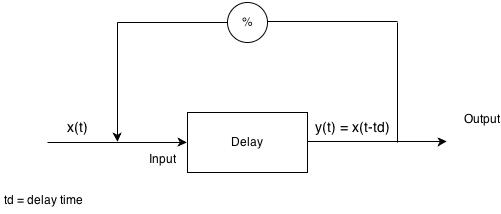
\includegraphics[height=120pt]{../pictures/image5.jpg}
\end{center}
\end{figure}
\newline \\ That percentage symbol is simply says that fraction of the signal is let through it.
So, in this case, the input is something like:
\newline \\ \texttt{x(t) + fraction*y(t)}
\newline \\And the output:
\newline \\ \texttt{x(t-td) + fraction*y(t-td)}
\section*{A Dry-wet Control}
In most audio applications, it is customary to have a control over how much of 
the sound effect is overlayed over the original sound. It is generally called a 
dry/wet control. Dry is the original sound. And wet is the sound effect.
It is just another simple 'percentage' thing again. Also, you throw in the original 
sound as well into the diagram. It looks something like this.
\begin{figure}[h]
\begin{center}
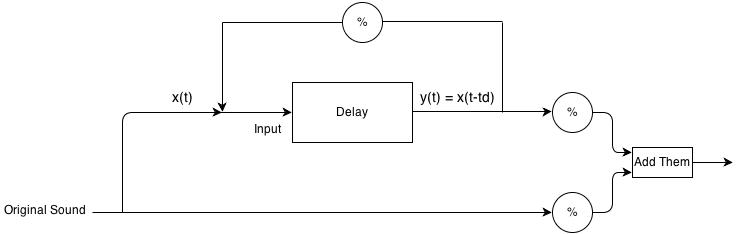
\includegraphics[height=120pt]{../pictures/image6.jpg}
\end{center}
\end{figure}
\section*{Why you should normalize Audio?}
An audio signal in the computer has this thing called the 'Dynamic Range'. 
All jargon aside, it dictates the limits within which the amplitude can be 
recognized as sound. For this particular library which we are using, it is from 
+1 to -1. So any values above (or below) these values would be brought back down 
to either -1 or +1. If this ever happens, you get this really noisy harsh sound. 
The only instances where this would happen is when you do addition operations like:
\newline \\ \texttt{x(t) + y(t)} 
Here, you should always normalize the audio i.e., average them. If you are using 
weights (like feedback, dry or wet) it is probably a good idea to do a weighted
average of the two sounds.
If you really want to know what that clipping noise (thats what it is called) 
sounds like, experiment a little and give it a listen. 
\end{document}

